\documentclass[a4paper]{book}
%\documentclass[a4paper]{ctexbook}
%\documentclass[a4paper]{ctexart}
\usepackage{ctex}
\usepackage{listings}
\usepackage{xcolor}
\usepackage{graphicx}
\usepackage{hyperref} %生成书签

%================================
% A.PDF标签
%================================
\hypersetup{
    colorlinks=true,
    bookmarksnumbered=true,
    pdftitle={My LaTeX2e note},
    pdfkeywords={LaTex, note},
}

\title{\Huge \bfseries 使用 \LaTeX 编写笔记}
\author{\huge 莫志烨}
\CTEXoptions[today=big]
\date{\Large \today}

%================================
% B.代码全局格式
%================================
\lstset{
    numbers=left,
    %numberstyle={\color{lightgray}},
    numberstyle={\color{green}},
    backgroundcolor={\color[RGB]{41, 47, 51}}, %背景颜色
    basicstyle={\color[RGB]{208, 214, 219}}, %普通字符串颜色
    stringstyle={\color[RGB]{0, 128, 0}}, %字符串颜色
    keywordstyle={\color[RGB]{101, 140, 230}}, %关键词颜色
    commentstyle={\color{gray}}, %注释颜色
    frame=none, %无边框
    breaklines=true, %自动分行
    language={[ANSI]C},
    captionpos=b,
}

%================================
% C.新命令定义
%================================

\newcommand{OutputListing}[]{
}

\begin{document}

%================================
% 1.标题
%================================
\chapter{标题}
\begin{titlepage}
\maketitle
\end{titlepage}

%================================
% 2.目录
%================================
\chapter{目录}
\tableofcontents

%================================
% 3.章节(每天日志入口)
%================================
\chapter{2020年3月2日 笔记}
\graphicspath{{note_everyday/001_20200302/picture/}}
\section{问题一:MMU学习}


1.步骤一:
\begin{figure}[h]
    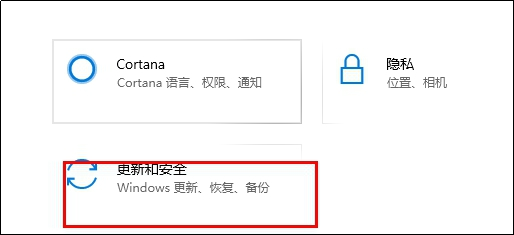
\includegraphics{001.jpg}
    \caption{第一步}
\end{figure}



\chapter{LaTex笔记}
\section{每天日志格式}

%1.每天日志格式

1.每天日志格式
\begin{lstlisting}[]
\chapter{2020年3月3日} //1.以日期为章节
\section{问题1} //2.以问题为小节!
\end{lstlisting}

2.插入代码格式1
\begin{lstlisting}[]
\begin{lstlistings}[caption={xxx}] %插入图注 //默认是C语法
\end{lstlistings}
\end{lstlisting}

2.插入代码格式2
\begin{lstlisting}[]
\lstinputlisting{lbuf.c}[caption={xxx}] %插入图注!
\end{lstlisting}

2.插入代码格式3
\begin{lstlisting}[]
\lstinline !code!
\end{lstlisting}

3.插入图片格式
\begin{lstlisting}[]
\graphicspath{{note_everyday/001_20200302/picture/}} %声明图片加载路径
\begin{figure}[h] %h:表示把图片放在当前位置
    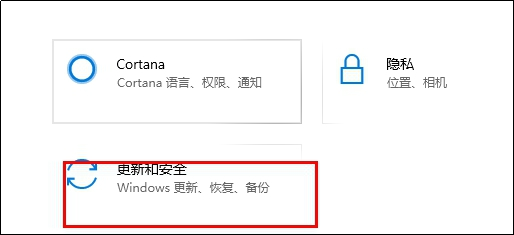
\includegraphics{001.jpg}
    \caption{第一步}
\end{figure}

\end{lstlisting}



\end{document}



%This is 日志.

